\subsection{Fact tracing for large language models (\mtfive)}
\label{subsec:fact_trace}
As large language models are deployed in a variety of contexts, e.g.,
as conversation agents \citep{thoppilan2022lamda}
or knowledge bases \cite{petroni2019language},
there is an emerging need to be able to
attribute models' outputs back to specific data sources
\cite{bohnet2022attributed}.
To that end, we study {\em fact tracing} \cite{akyurek2022towards}, i.e.,
the task of identifying the training examples that cause a language model to
generate a given ``fact.''

\paragraph{A benchmark for fact tracing.}
\citet{akyurek2022towards} develop a testbed for the fact tracing problem
by way of a dataset (and corresponding evaluation methodology) called \ftracetrex.
We provide a high-level overview of \ftracetrex here,
and describe it in more depth in \cref{app:fact_tracing:dataset}.
The \ftracetrex dataset consists of a set of ``abstracts'' and a set
of ``queries,'' both of which pertain to the same database of
``facts.''
\citet{akyurek2022towards} annotate each abstract
with a set of facts it expresses, and
each query with the (single) fact that it asks about.
As a part of the task setup, one finetunes a pre-trained language model on the set
of abstracts using {\em masked language modeling},\footnote{
In masked language modeling \citep{raffel2020exploring}, the language model is asked to predict the tokens
corresponding to a masked-out portion of the input. In \ftracetrex, either a subject or object in the abstract is masked out.}
and then evaluates this model's correctness on each query in
the query set.
This step defines a set of ``novel facts,'' i.e.,
queries that the model answers correctly {\em only after} finetuning.

With the above setup in place, we can define the \ftracetrex fact tracing benchmark.
\citet{akyurek2022towards} reason that each novel fact (as identified above)
should have been learned (during finetuning) from the abstracts that express the same fact.
The benchmark thus evaluates a given data
attribution method's ability to retrieve, for each novel fact,
the abstracts in the training set that express the same fact.
(Such abstracts are called the {\em ground-truth proponents} of the query.)

In particular, observe that applying a data attribution method $\tau(\cdot)$ to
a particular query (treating the set of abstracts as the training set) yields
scores that we can use as a ranking over the set of the abstracts.
\citet{akyurek2022towards} compute the {\em mean reciprocal rank} (MRR)
of the ground-truth proponents in this ranking (see \cref{app:fact_tracing:dataset}),
a standard metric from information retrieval,
to quantify the efficacy of $\tau(\cdot)$ at fact tracing.
We evaluate \trak on this benchmark,
along with two baselines from
\citep{akyurek2022towards}, \tracin \cite{pruthi2020estimating}
and the information retrieval method BM25 \cite{robertson1995okapi}.

\paragraph{Computing \trak scores for language models.}
To apply \trak to this setting, we need to choose an appropriate model output function,
as we did before for the classification setting (see \Cref{ssec:multiclass}) and for \clip (see \Cref{sec:CLIP}).
To this end, we observe that the  masked language modeling objective
has a natural interpretation as a sequence of $v$-way classification problems over the masked tokens,
where $v$ is the vocabulary size. %
Thus, inspired by our analysis of the multi-class classification setting
from \cref{ssec:multiclass}, %
we choose the model output function for this setting to be
the sum of the ``canonical'' model output function \eqref{eq:modelout_mc}
for each of the $v$-way classification problems
(see \cref{app:fact_tracing:trak} for more details).

\subsubsection{Results and discussion}
We find that while \trak significantly outperforms \tracin on
the \ftracetrex benchmark (0.42 vs. 0.09 using the aforementioned MRR score),
neither method matches the
performance of the information retrieval baseline BM25 (0.77 MRR).\footnote{Note that
while our finding that BM25 outperforms \tracin
matches that of \citet{akyurek2022towards}, our exact numbers are incomparable
due to the mismatch in model classes.}

To understand the possible roots of \trak's underperformance
relative to BM25 on \ftracetrex,
we carry out a counterfactual analysis.\footnote{
    See \cref{app:fact_tracing:cfx} for a detailed account of our experiment.
}
Specifically, for a subset $S^\star$ of the \ftracetrex query set, we
create three corresponding {\em counterfactual training sets}.
Each such training set corresponds to {\em removing} one of three collections of abstracts
from the \ftracetrex abstract set:
\begin{enumerate}
    \item[(a)] the most important abstracts for model performance on $S^\star$, as estimated by \trak;
    \item[(b)] the abstracts that are most similar to the queries in $S^\star$ according to BM25;
    \item[(c)] the corresponding ``ground-truth proponents'' for the queries in $S^\star$ as per \ftracetrex.
\end{enumerate}
We then measure the average {\em decrease} in performance on $S^\star$ when a model is finetuned on these
counterfactual datasets compared finetuning on the full training set.
Intuition would suggest that performance would decrease the most when models are
trained on the counterfactual training set~(c); in particular,
there is ostensibly {\em no} direct evidence for {\em any} of the facts corresponding to the queries in $S^\star$
anywhere in that set.

We find (see \cref{fig:nlp_counterfactual}), however, that it is
only the \trak-{\em based counterfactual training set} that
causes a large change in model behavior.
That is, removing abstracts identified with \trak
leads to a 34\% decrease in accuracy,
significantly more than the decreases induced by removing abstracts according to
BM25 (10\%) or even removing {\em ground-truth proponents} (12\%).

\begin{figure}[h]
    \centering
    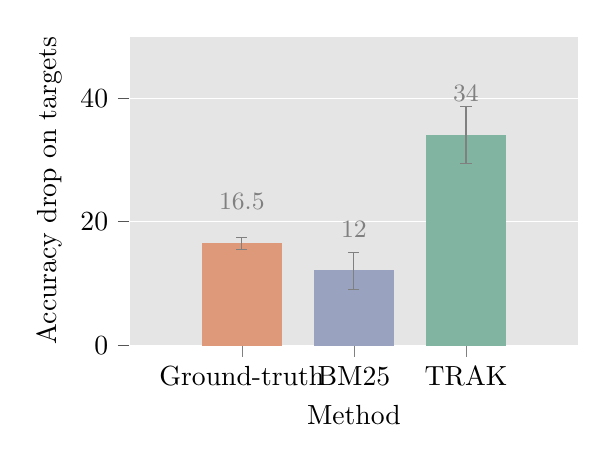
\begin{tikzpicture}
    \definecolor{darkgray141160203}{RGB}{141,160,203}
    \definecolor{dimgray85}{RGB}{85,85,85}
    \definecolor{gainsboro229}{RGB}{229,229,229}
    \definecolor{lightgray204}{RGB}{204,204,204}
    \definecolor{mediumaquamarine102194165}{RGB}{102,194,165}
    \definecolor{orchid231138195}{RGB}{231,138,195}
    \definecolor{salmon25214198}{RGB}{252,141,98}
    \definecolor{amethyst}{rgb}{0.6, 0.4, 0.8}
    \definecolor{bleudefrance}{rgb}{0.19, 0.55, 0.91}
    \definecolor{blush}{rgb}{0.87, 0.36, 0.51}
    \definecolor{brilliantrose}{rgb}{1.0, 0.33, 0.64}
    \definecolor{trakorange}{rgb}{0.87, 0.6, 0.48}
    \definecolor{trakgreen}{rgb}{0.51, 0.705, 0.635}
    \definecolor{trakblue}{rgb}{0.60, 0.64, 0.753}
    \begin{axis}[
        axis background/.style={fill=gainsboro229},
        axis line style={white},
        width=0.6\textwidth,
        height=5.5cm,
        ybar,
        tick align=outside,
        tick pos=left,
        enlarge x limits=0.5,
        ylabel={Accuracy drop on targets},
        xlabel={Method},
        xtick={1,2,3},
        xticklabels={Ground-truth, BM25, TRAK},
        nodes near coords={
            \pgfmathprintnumber[fixed]{\pgfplotspointmeta}
        },
        nodes near coords style={
            yshift=0.3cm,
            text=gray,
            font=\small
        },
        nodes near coords align={vertical},
        ymin=0,
        ymax=1, %
        error bars/y dir=both,
        error bars/y explicit,
        error bars/error bar style={gray},
        bar width={1cm},
        y grid style={white},
        ymajorgrids,
        ymin=0, ymax=50,
        ytick style={color=dimgray85}
        ]
        \addplot[fill=trakorange,
                  draw=trakorange, 
                  bar shift=0cm,
                  error bars/.cd, 
                  y dir=both, 
                  y explicit]
            coordinates{
                (1, 16.5) +- (0, 1)%
            }; 
        
        \addplot[fill=trakblue, 
                  draw=trakblue,
                  error bars/.cd, 
                  y dir=both, 
                  y explicit]
            coordinates {
                (2, 12) +- (3.0, 3.0)
            }; 

        \addplot[fill=trakgreen, 
                  draw=trakgreen,
                  bar shift=0cm,
                  error bars/.cd, 
                  y dir=both, 
                  y explicit]
            coordinates {
                (3, 34) +- (4.8, 4.6)
            }; 
    \end{axis}
\end{tikzpicture}
\caption{{\em Identifying counterfactually important examples for learning facts on \ftracetrex.}
        Given a set of queries that the language model (\texttt{mt5-small}) originally answers correctly after training, we compare how three different interventions---removing abstracts with the highest \trak scores, removing the most similar abstracts according to BM25, and removing the ground-truth proponents as indicated by \ftracetrex---affect the resulting model's accuracy on the queries.
        The $y$-axis shows the {\em decrease} in accuracy (on the query set, relative to the original model) after each intervention; results are averaged over 50 queries and eight independent models.
        Error bars represent $95\%$ confidence intervals.
    }
    \label{fig:nlp_counterfactual}
\end{figure}

\paragraph{Discussion.}
Our results demonstrate that while \trak may not be effective at identifying abstracts
that directly express the same fact as a given query
(i.e., the ground-truth proponents as defined by \ftracetrex),
it {\em can} successfully identify the abstracts that are most
responsible for the finetuned model {\em learning} a given fact.
In particular, \trak's subpar performance on the attribution benchmark
is an artifact of the \ftracetrex benchmark rather than a flaw of \trak itself.

There are several potential explanations for this phenomenon, many of which
\citet{akyurek2022towards} already discuss in their work:
\begin{itemize}
    \item There may be errors in the \ftracetrex benchmark. (Although,
    given the drastic difference between the \trak scores
    and the ground-truth labels in their ability to identify counterfactually important abstracts,
    such data errors are unlikely to be the sole culprit.)
    \item Models may be answering queries by
    {\em combining} facts from the training set.
    For example, neither ``The largest pyramid is in Giza'' nor ``Giza is a city in Egypt'' would be
    ground-truth proponents for the query ``Which country is home to the largest pyramid?'' in \ftracetrex,
    but a model that learns both of these facts
    may still be able to correctly answer that query.
    \item Alternatively, models may be learning from the syntactic rather than
    semantic structure of abstracts. For example, a model may correctly answer
    that a person from Korea is called a ``Korean'' by learning from an
    abstract which says ``A person from Bulgaria is Bulgarian.''
\end{itemize}

More broadly,
our results highlight a difference between {\em fact tracing}
and {\em behavior tracing}.
In other words,
finding a data source that supports a given model-generated text is a different task
than identifying the actual data sources that {\em caused} the model to generate this text in
the first place.
While we may be able to address the former problem with { model-independent}
techniques such as information retrieval or web search,
the latter requires methods that remain faithful to (and thus, dependent on)
the model being studied. Our results here indicate that \trak can be an effective tool for the latter problem.









